
\documentclass {article}
\usepackage{graphicx}
\usepackage[hypcap]{caption}
\usepackage{amssymb,amsmath}
\begin{document}
\title{CSE603 Assignment2}
\author {Ruhan Sa 50060400}
\maketitle
\noindent \textbf{Aim}: Compute the product of matrix A and matrix B. Result stored into C.

\noindent \textbf{Input}: Both A and B are generated using dynamic allocation, using malloc function in C. Size of A and B are determined in the command line as input argument of main function. In normal experiment phases, the element is derived from random float numbers ranges from 0 to 2.

\noindent \textbf{Verification}:  This is done using matrix with unit elements and the result is verified by checking wether elements of C equals to the matrix size or not. If so the implementation is verified, if not the implementation is wrong.

\noindent \textbf{Maximum matrix size}: The maximum matrix size here denotes the maximum matrix size whose time consumption is still observable during the assignment cycle. The walltime of CCR are within 24 hours in all experiments below.

\noindent \textbf{Compilation}: All the compilations are done using following script  in the CCR front-end.
\begin{figure}[htp!]
\centering
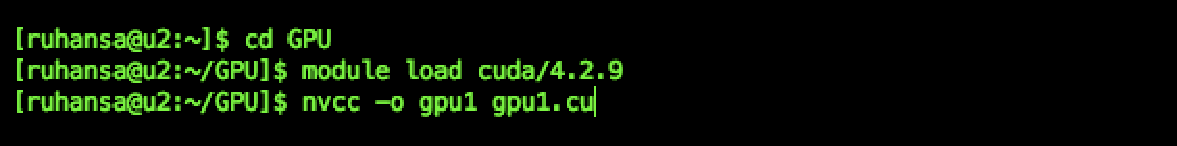
\includegraphics[width = \linewidth]{nvcc.pdf}
\caption{Compilation script}
\label{fig:nvcc}
\end{figure}

\section{One block with one thread per element}

\begin{figure}[htp!]
\centering
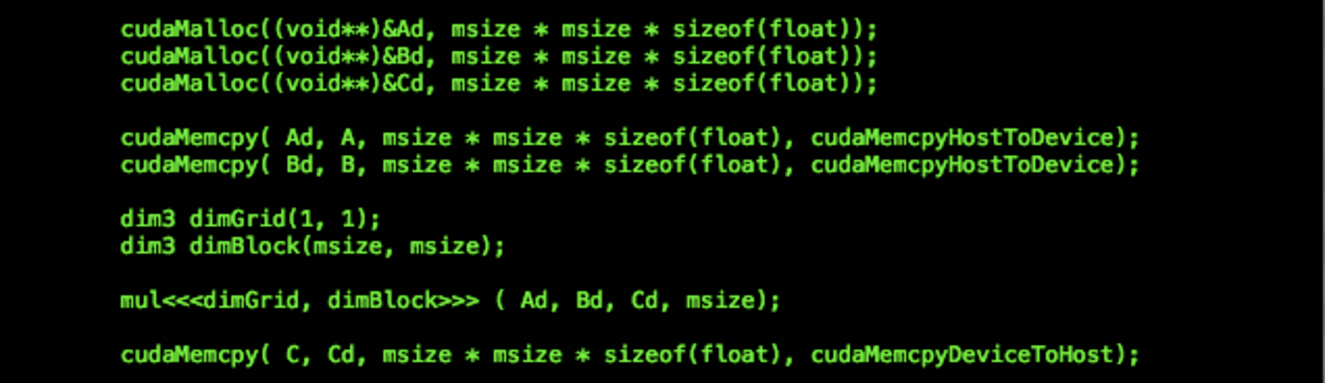
\includegraphics[width = \linewidth]{gpu11.pdf}
\caption{Host side code}
\label{fig:one}
\end{figure}

\begin{figure}[htp!]
\centering
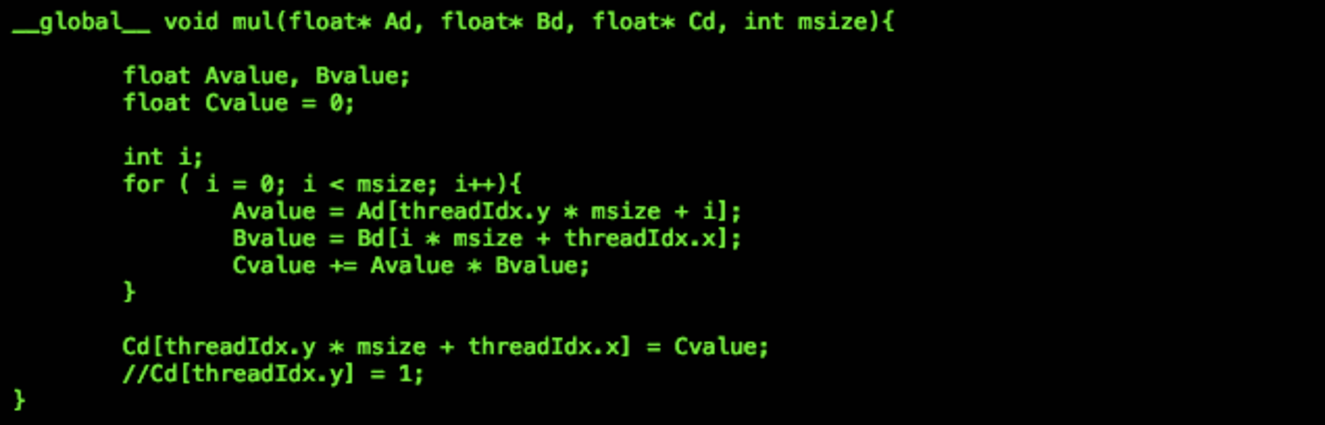
\includegraphics[width = \linewidth]{gpu12.pdf}
\caption{Device side code}
\label{fig:two}
\end{figure}

\begin{figure}[htp!]
\centering
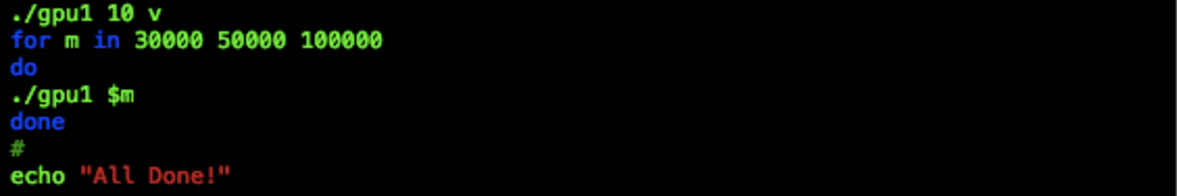
\includegraphics[width = \linewidth]{gpu13.pdf}
\caption{partial script}
\label{fig:three}
\end{figure}

\subsection{A Glimpse of Source Code}

Main part of the source code and the scripts are shown in Figure 2 and Figure 3. In this part, the block size is determined by the matrix size, which is denoted as variable $"msize"$ in the code. Threads within one block is scaled in $msize \times msize$ fashion. 

The script shows the command line of running verification as well as the experiments on CCR. As Figure 4 shows the matrix size is determined in the command line. This way the code can be more flexible than defining the size in the code. 

\subsection{Result with the increase of matrix size}

\begin{figure}[htp!]
\centering
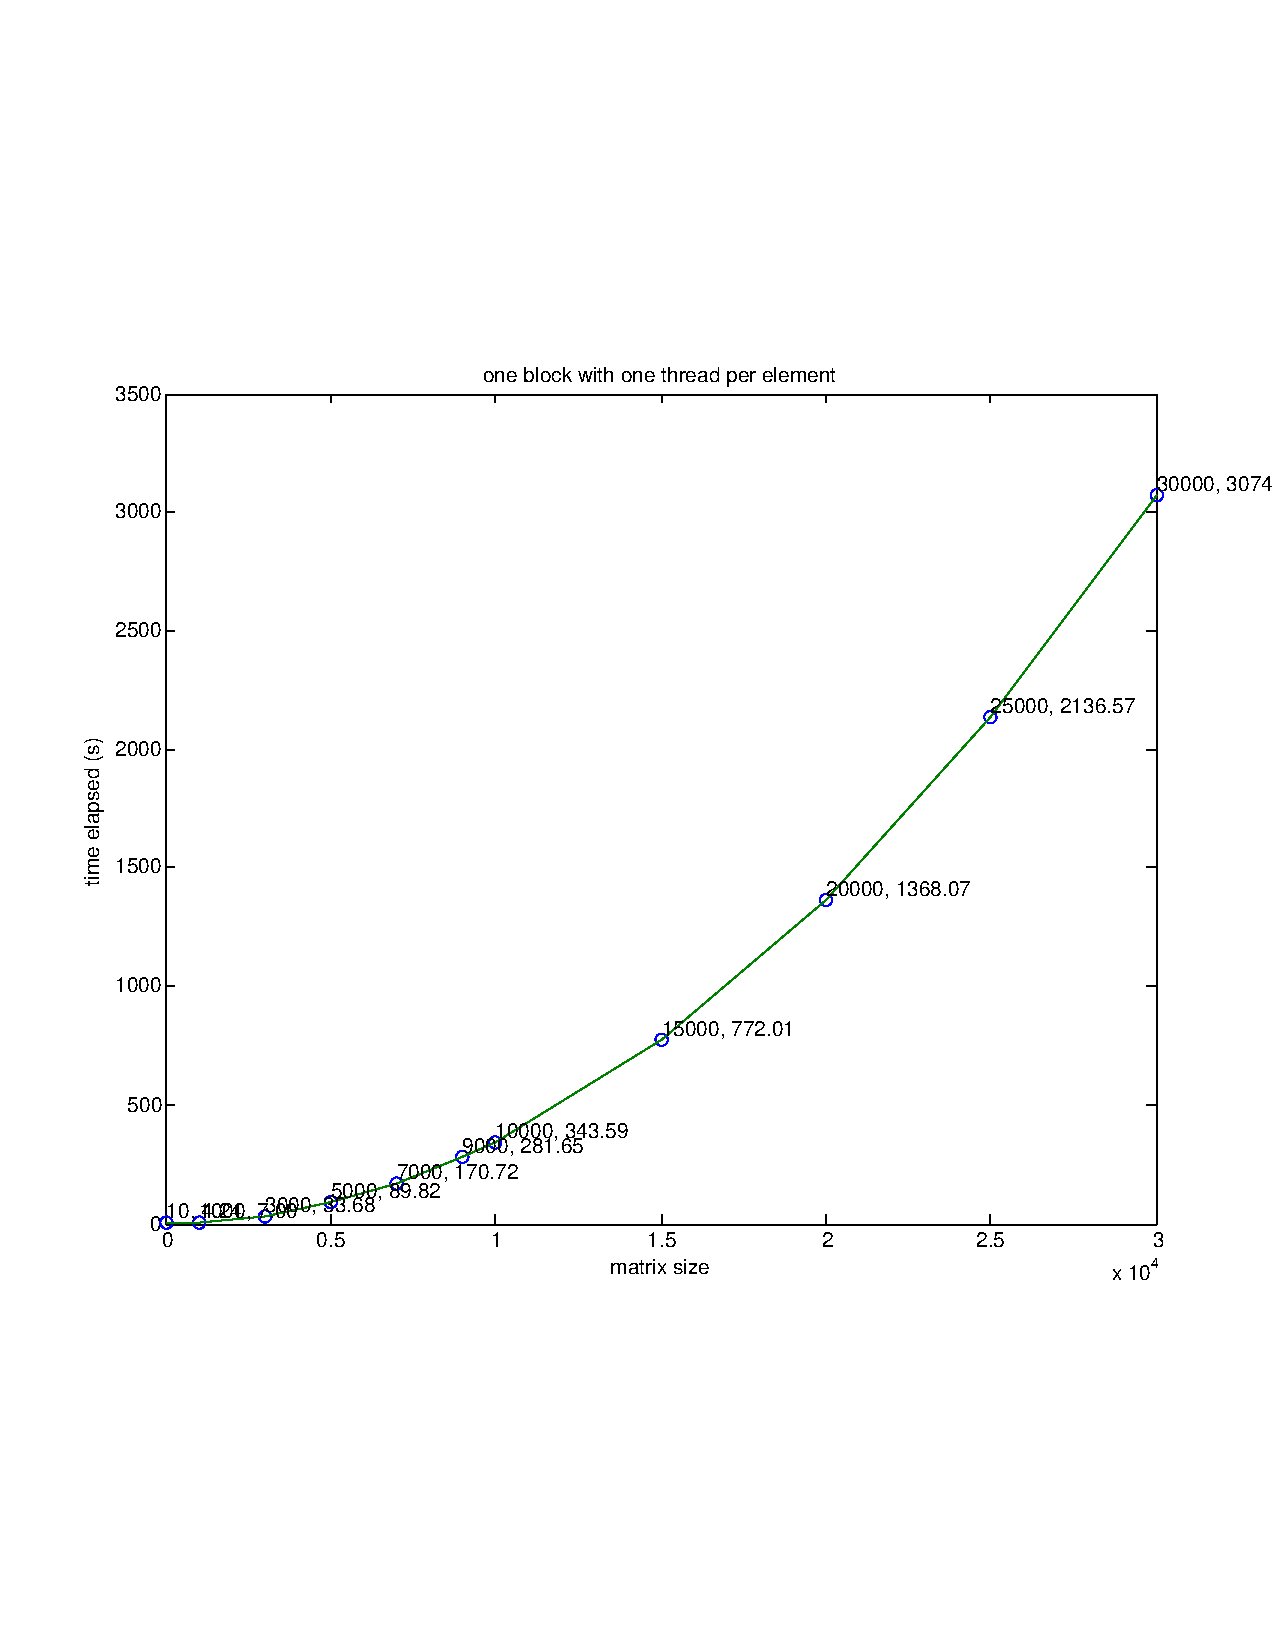
\includegraphics[width=0.8\linewidth]{r_gpu11.pdf}
\caption{time consumption with the increase of matrix size.}
\label{fig:four}
\end{figure}

Figure 5 shows the time consumption with the increase of matrix size. The maximum matrix size is $30000 \times 30000$.

\section{Multiple blocks with one thread per element}
\subsection{A Glimpse of Source Code}
Main part of the source code and the scripts are shown in Figure 6, Figure 7 and Figure 8. As the code shows, every block solves $tile \times tile$ elements and are layed out uniformly in the Grid. Each element are solved by one thread.

\begin{figure}[htp!]
\centering
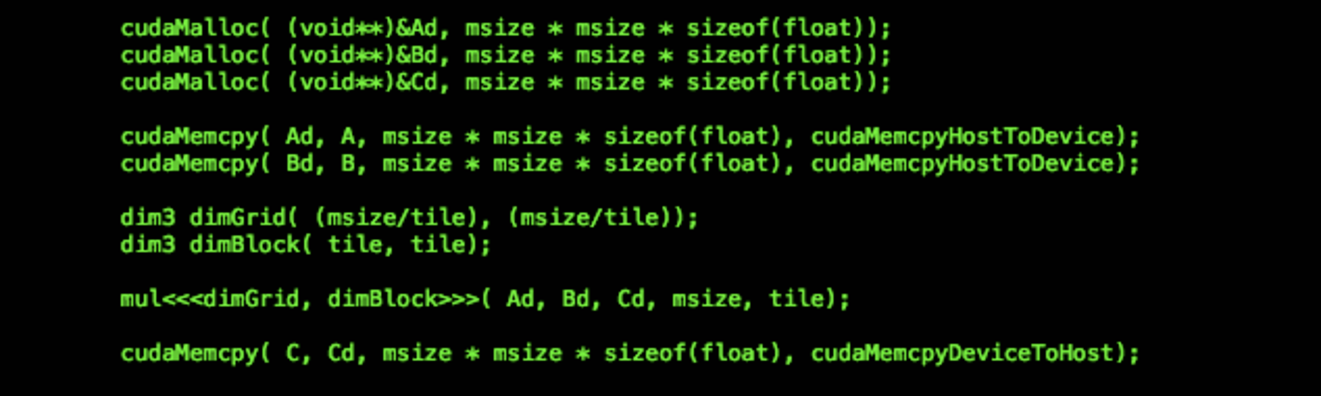
\includegraphics[width = \linewidth]{gpu21.pdf}
\caption{Host side code}
\label{fig:gpu21}
\end{figure}

\begin{figure}[htp!]
\centering
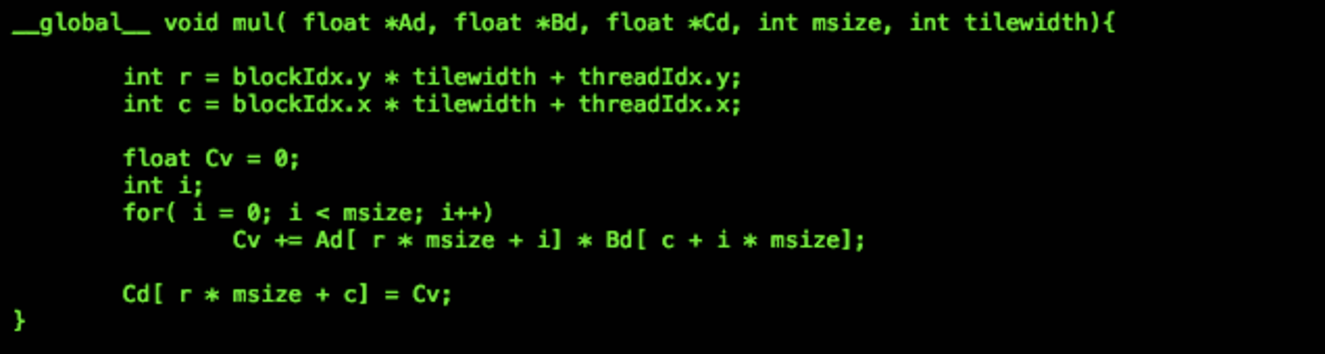
\includegraphics[width = \linewidth]{gpu22.pdf}
\caption{Device side code}
\label{fig:gpu22}
\end{figure}

\begin{figure}[htp!]
\centering
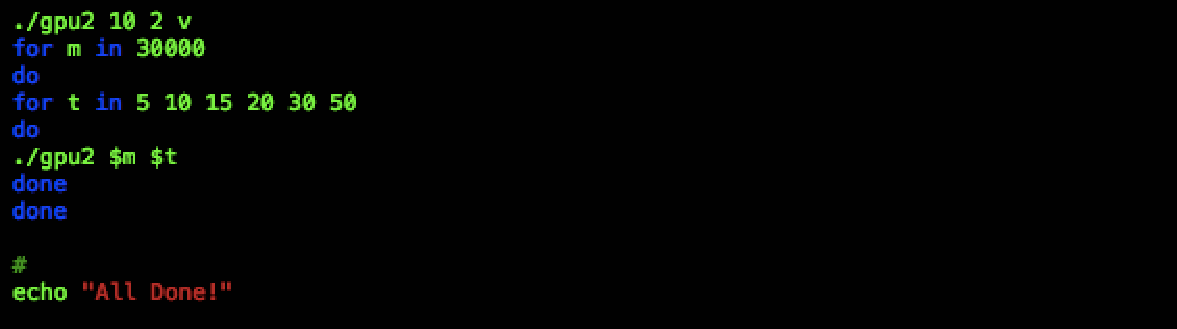
\includegraphics[width = \linewidth]{gpu23.pdf}
\caption{partial script}
\label{fig:gpu23}
\end{figure}

\subsection{Result with the increase of matrix size}
\begin{figure}[htp!]
\centering
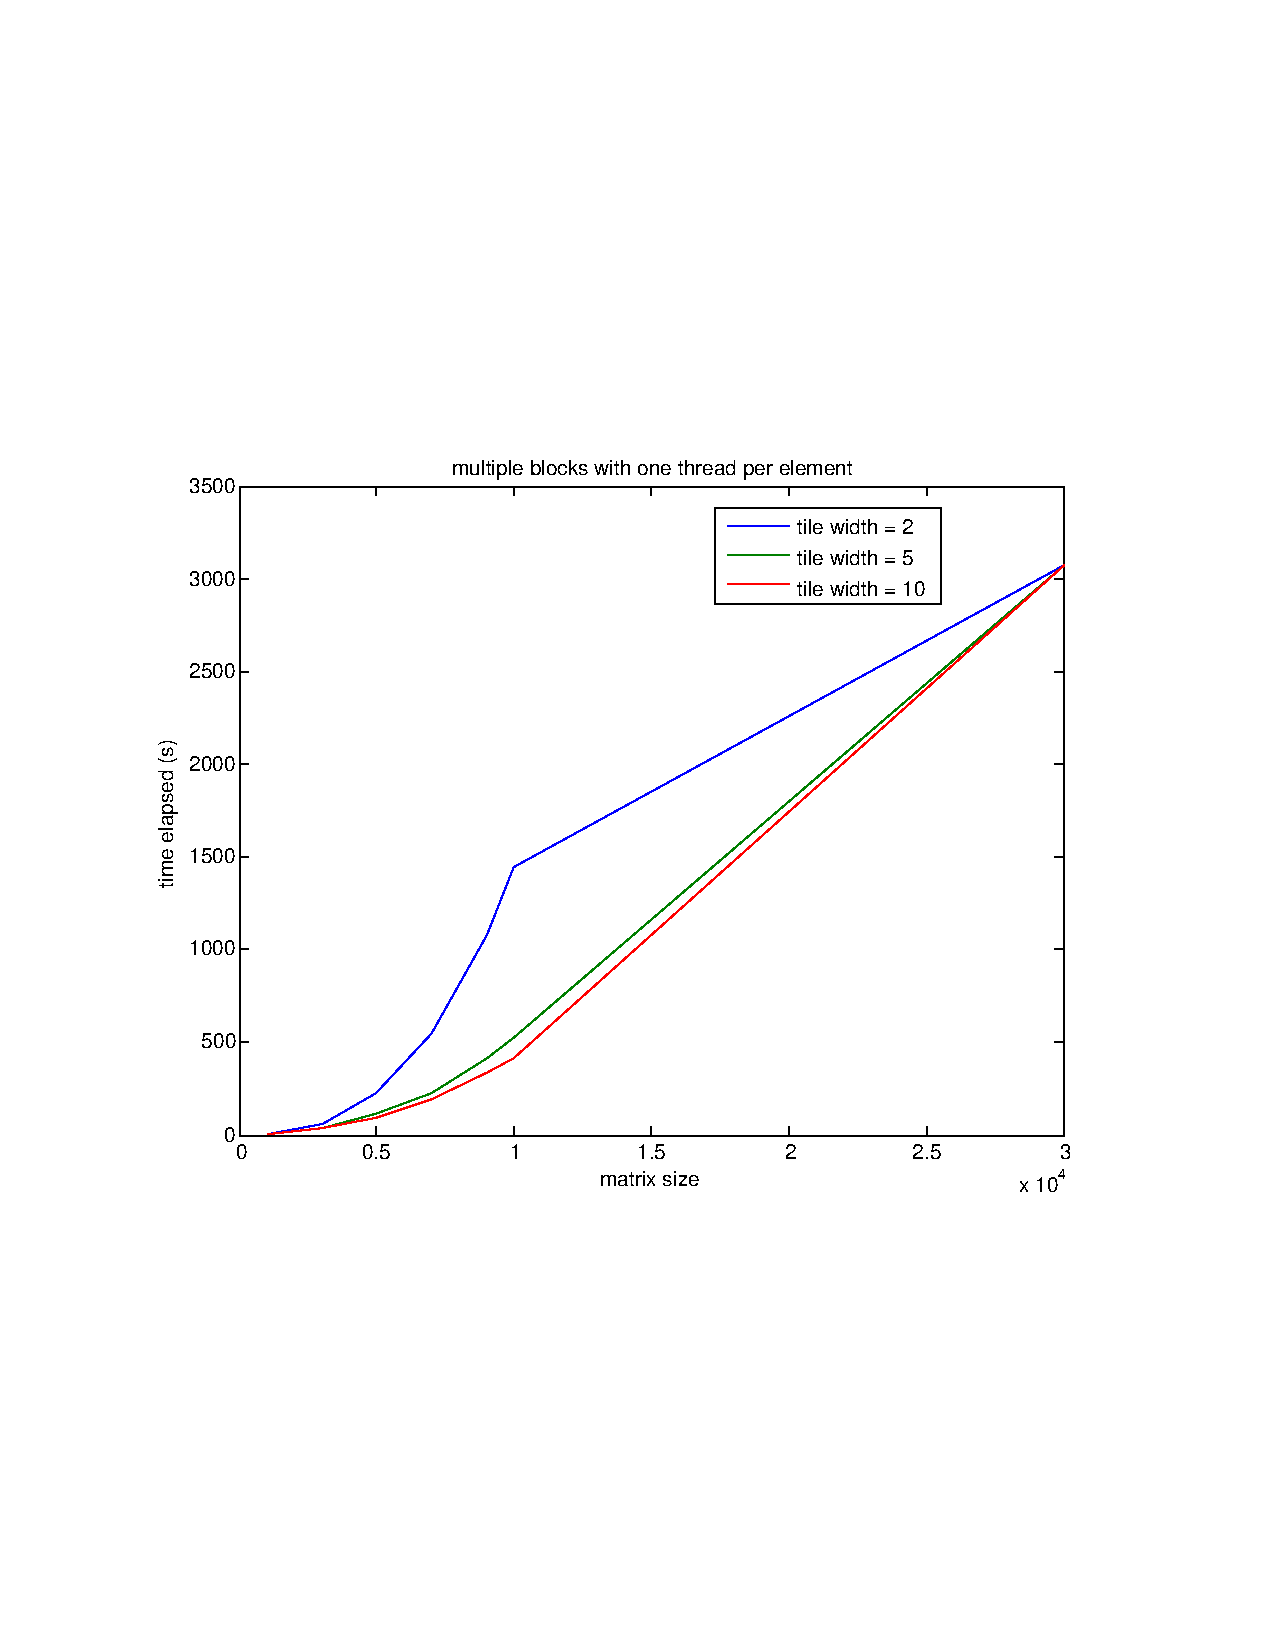
\includegraphics[width=0.8\linewidth]{r_gpu21.pdf}
\caption{time consumption with the increase of matrix size.}
\label{fig:rgpu2}
\end{figure}

Figure 9 shows the time consumption with the increase of matrix size. The maximum matrix size is $30000\times 30000$. Since, in this part, the time consumption can be influenced by 2 major facts: size of the matrix and the tile width. The experiments are conducted using different $"tile\_width"$ chosen from $\{2, 5, 10\}$. From the figure we can see that with the increase of tile\_width, \textit{i.e.} with the increase of the number of elements solved by per block, the speed goes up. For example when computing $1000 \times 1000$ matrix, the time consumption of using $2\times2$ elements per block is three times larger than using $10\times10$ elements per block. This is because, one SM can only take 8 blocks, if the granularity is 4 thread/block, the whole SM only reaches $(4 * 8 = 32)$ threads. However if the granularity is 100 thread/block, one SM can hold all blocks, which means that one SM can compute up to 768 (which is the whole capacity according to G80) threads simultaneously.
\section{Multiple blocks with one thread multiple element}

\begin{figure}[htp!]
\centering
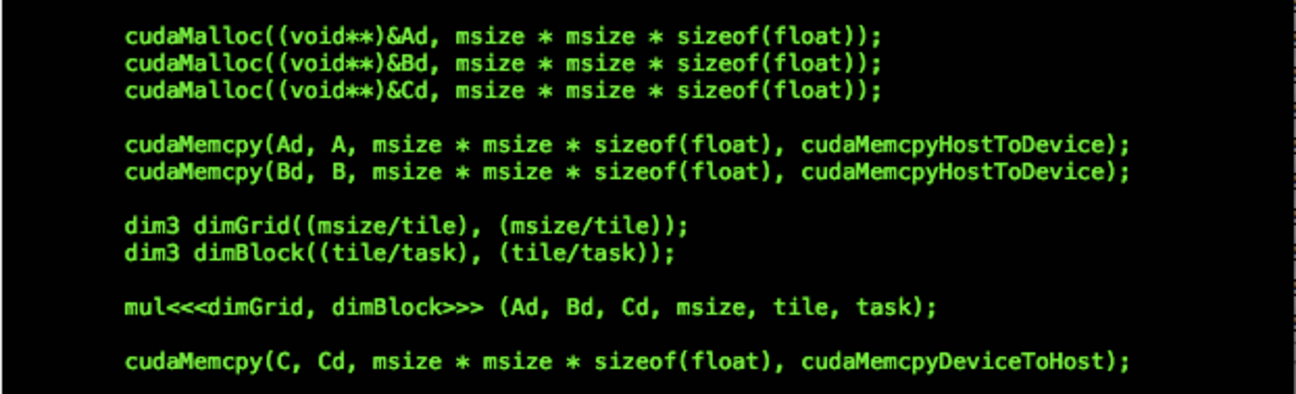
\includegraphics[width = \linewidth]{gpu31.pdf}
\caption{Host side code}
\label{fig:gpu31}
\end{figure}

\begin{figure}[htp!]
\centering
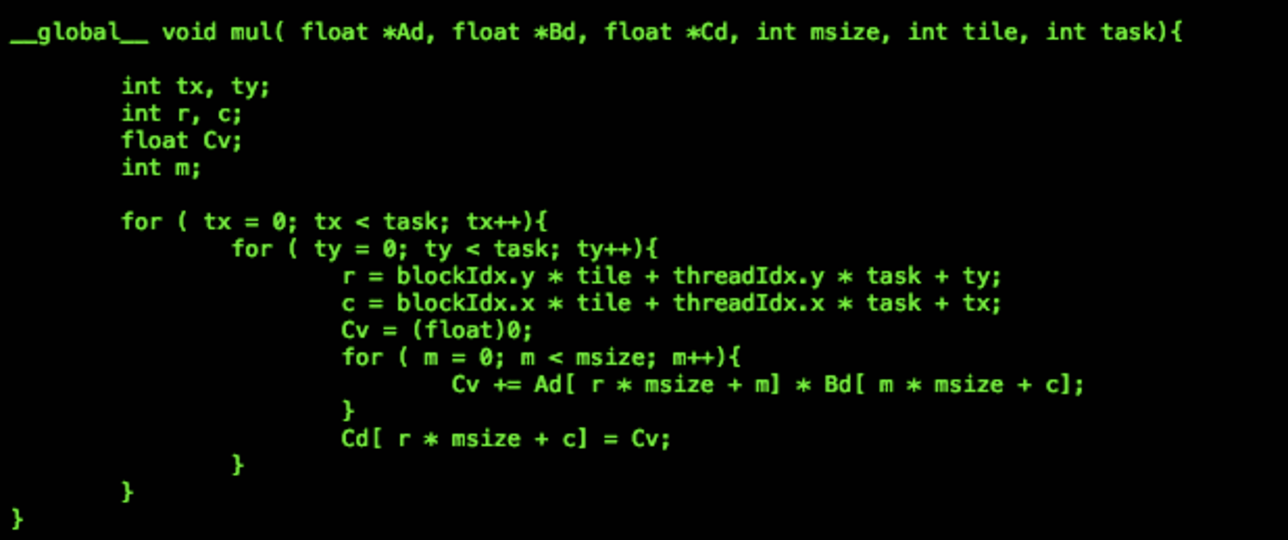
\includegraphics[width = \linewidth]{gpu32.pdf}
\caption{Device side code}
\label{fig:gpu32}
\end{figure}
\subsection{A Glimpse of Source Code}
Main part of the source code and the scripts are shown in Figure 10, Figure 11 and Figure 12. As the code shows, block granularity here is determined by $tile \times tile$ and each thread solves $task \times task$ elements. 

\begin{figure}[htp!]
\centering
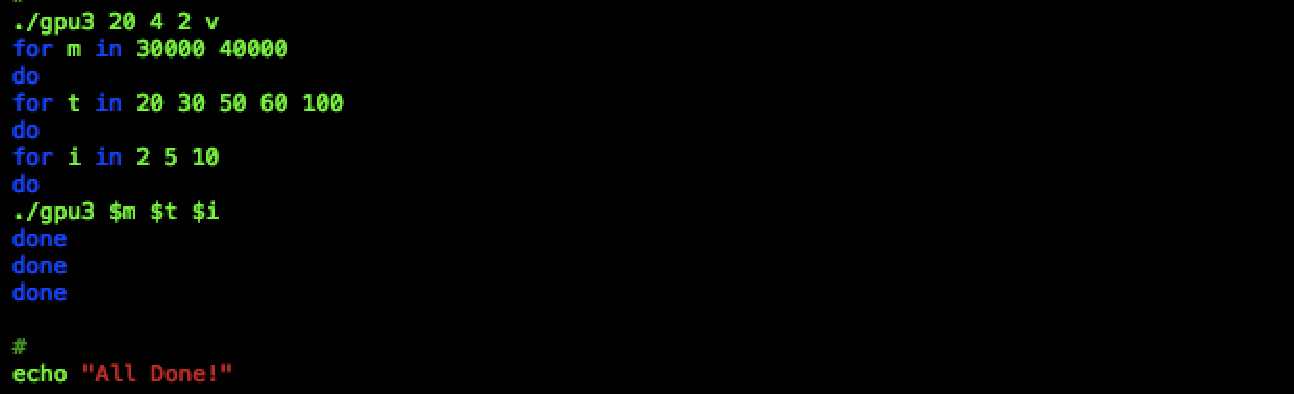
\includegraphics[width = \linewidth]{gpu33.pdf}
\caption{partial script}
\label{fig:gpu33}
\end{figure}

\begin{figure}[htp!]
\centering
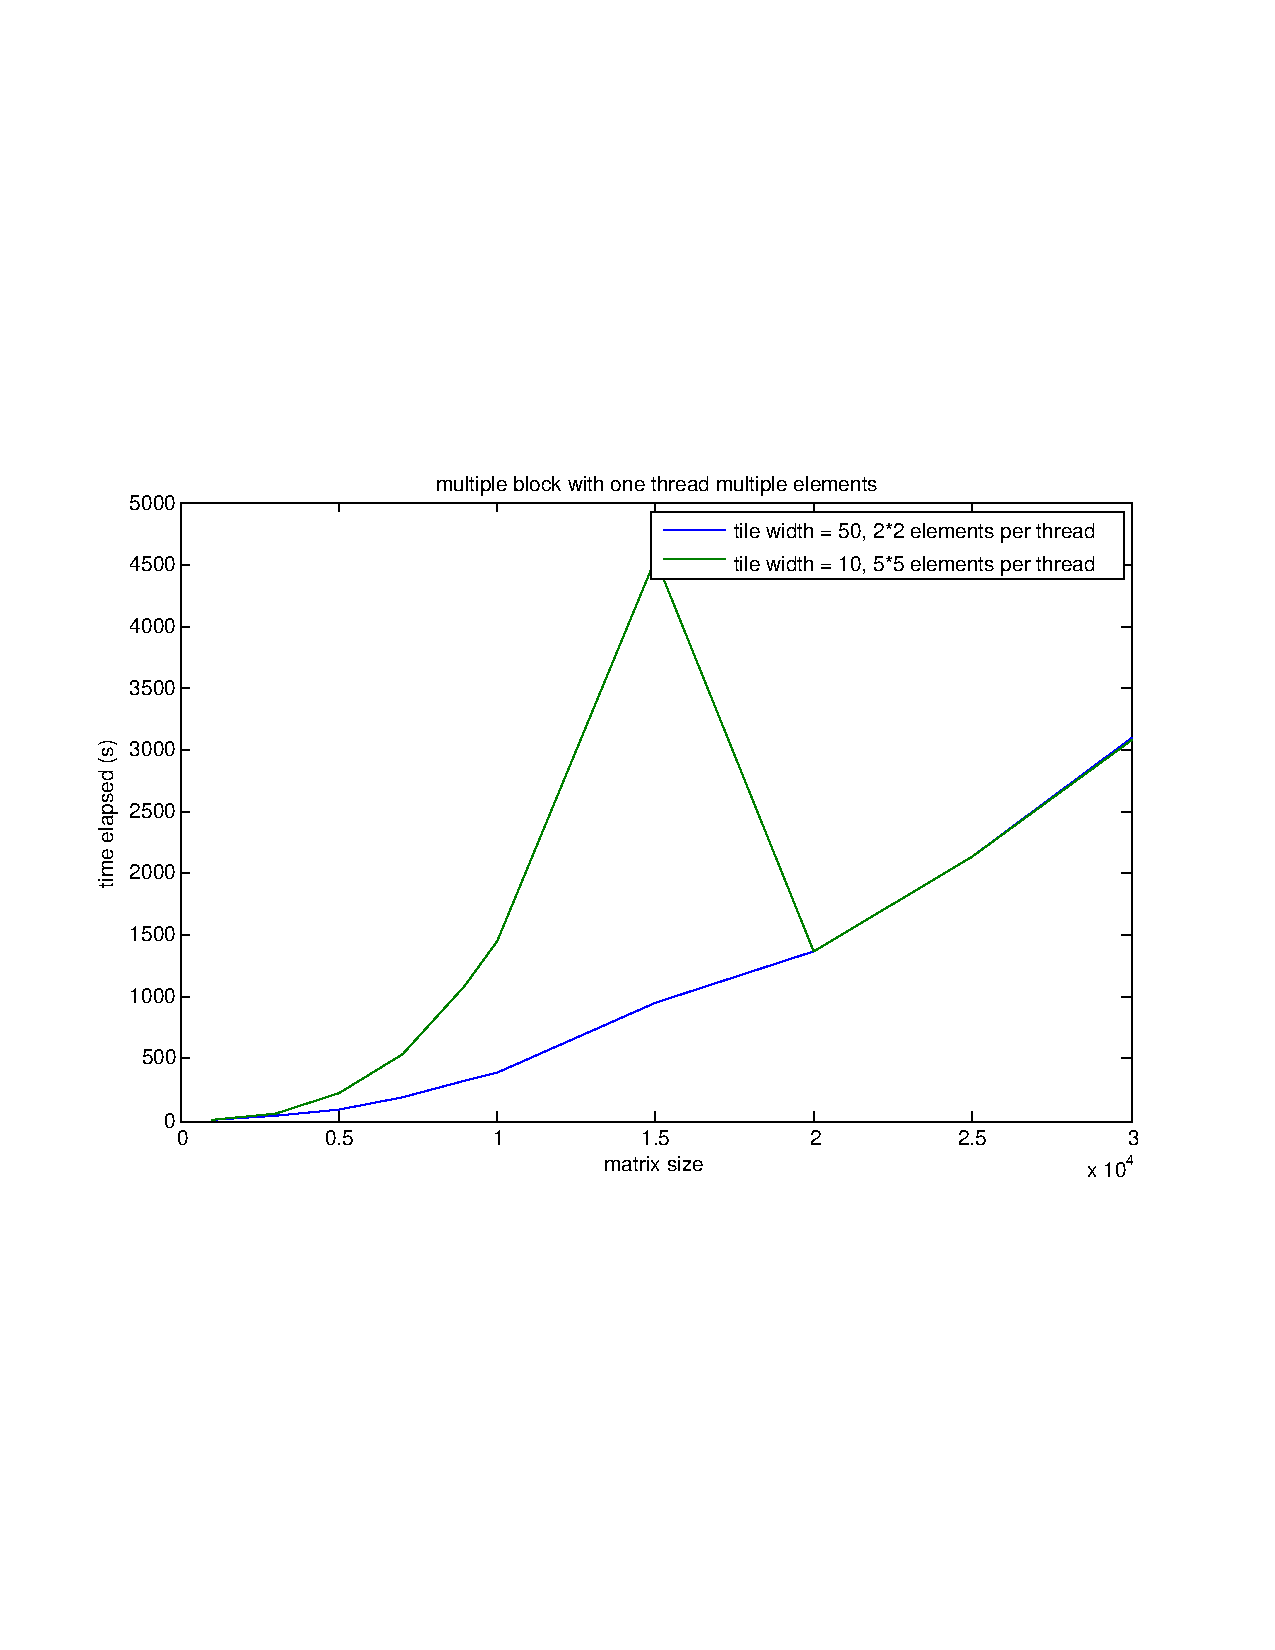
\includegraphics[width = 0.8\linewidth]{r_gpu31.pdf}
\caption{time consumption with the increase of matrix size}
\label{fig:rgpu3}
\end{figure}


\subsection{Result with the increase of matrix size}
In this part the time consumption is determined by three factors, matrix size, the tile\_width and the task\_width. The experiments tries to cover different parameters to see the effect. The tile\_width is chosen from $\{10, 20, 50\}$ and the task\_width is chosen from $\{2, 5, 10\}$. Since the data is too much to plot in one figure, Figure 13 shows only the two extreme cases, the fastest one, which has $50 \times 50$ tile and $2 \times 2$ elements per thread granularity, and the slowest one, which has $10 \times 10$ tile and $5 \times 5$ elements per thread granularity. However, when the matrix size exceeds $2000 \times 2000$, the time consumptions of all granularity are similar. The maximum matrix size here is $30000 \times 30000$.
\section{Double Buffering}

\begin{figure}[htp!]
\centering
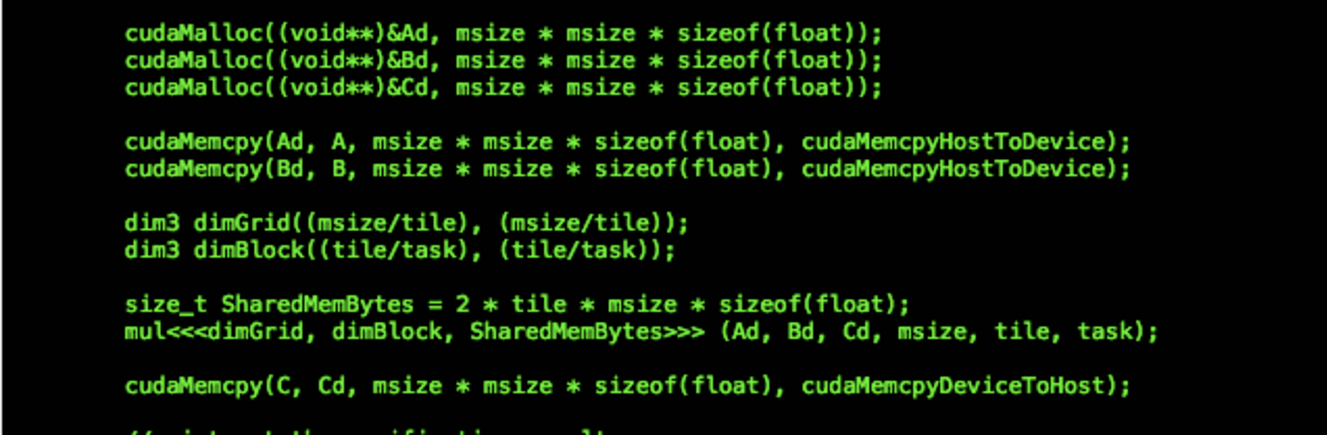
\includegraphics[width = \linewidth]{gpu41.pdf}
\caption{Host side code}
\label{fig:gpu41}
\end{figure}

\begin{figure}[htp!]
\centering
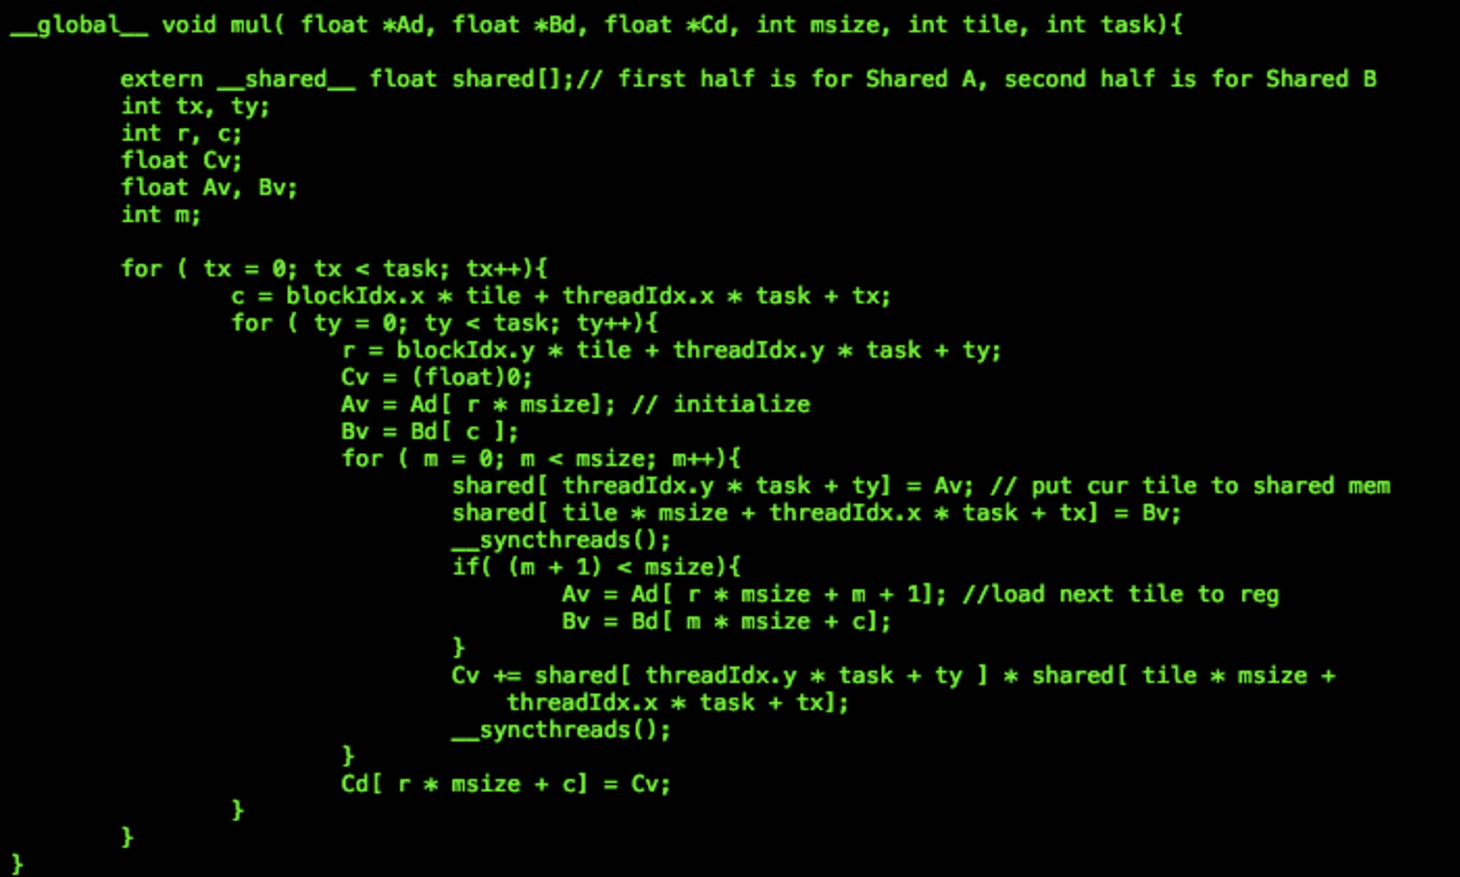
\includegraphics[width = \linewidth]{gpu42.pdf}
\caption{Device side code}
\label{fig:gpu42}
\end{figure}

\subsection{A Glimpse of Source Code}
Main part of the source code and the scripts are shown in Figure 14, Figure 15 and Figure 16. The Device side code shows that the double buffering is accomplished by simultaneously reading and computing, \textit{i.e.} read the next tile and compute the current tile simultaneously.

\begin{figure}[htp!]
\centering
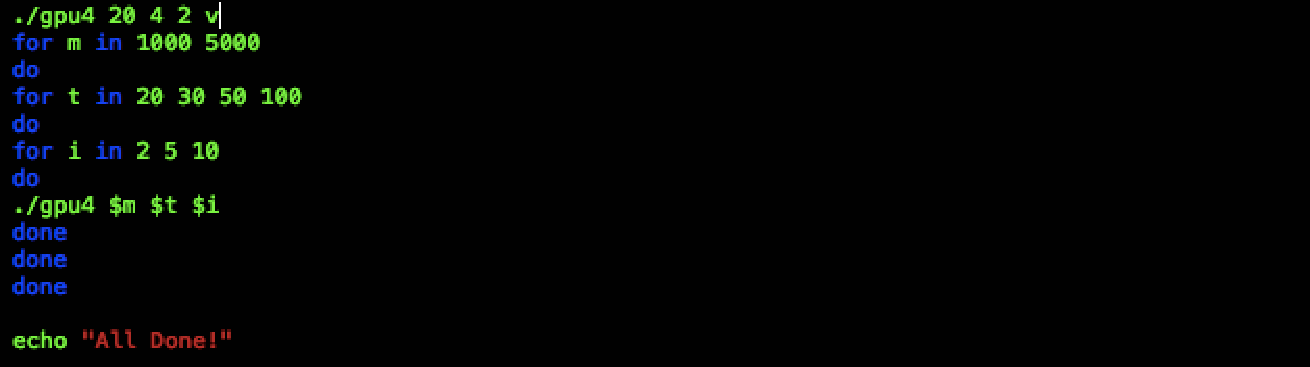
\includegraphics[width = \linewidth]{gpu43.pdf}
\caption{partial script}
\label{fig:gpu43}
\end{figure}

\begin{figure}[htp!]
\centering
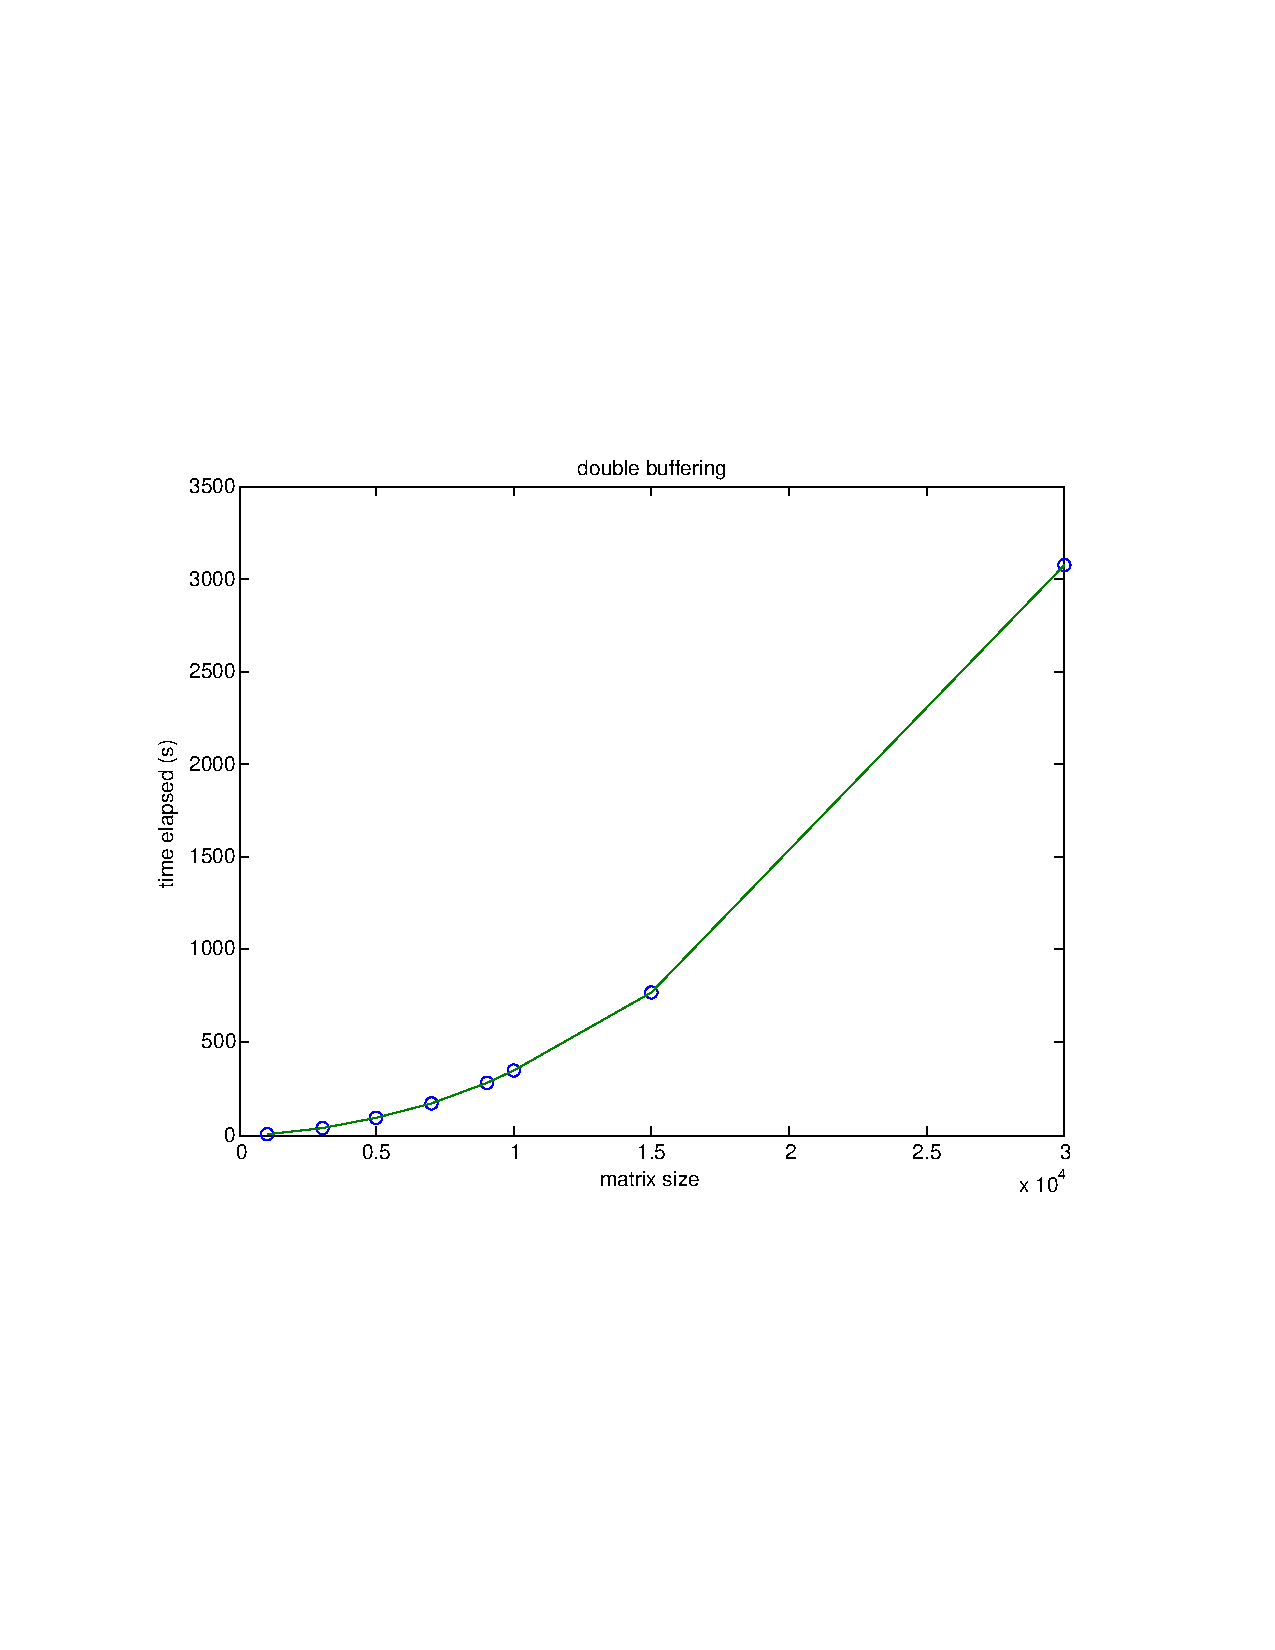
\includegraphics[width = \linewidth]{r_gpu41.pdf}
\caption{time consumption with the increase of matrix size}
\label{fig:rgpu4}
\end{figure}

\begin{figure}[hbp!]
\centering
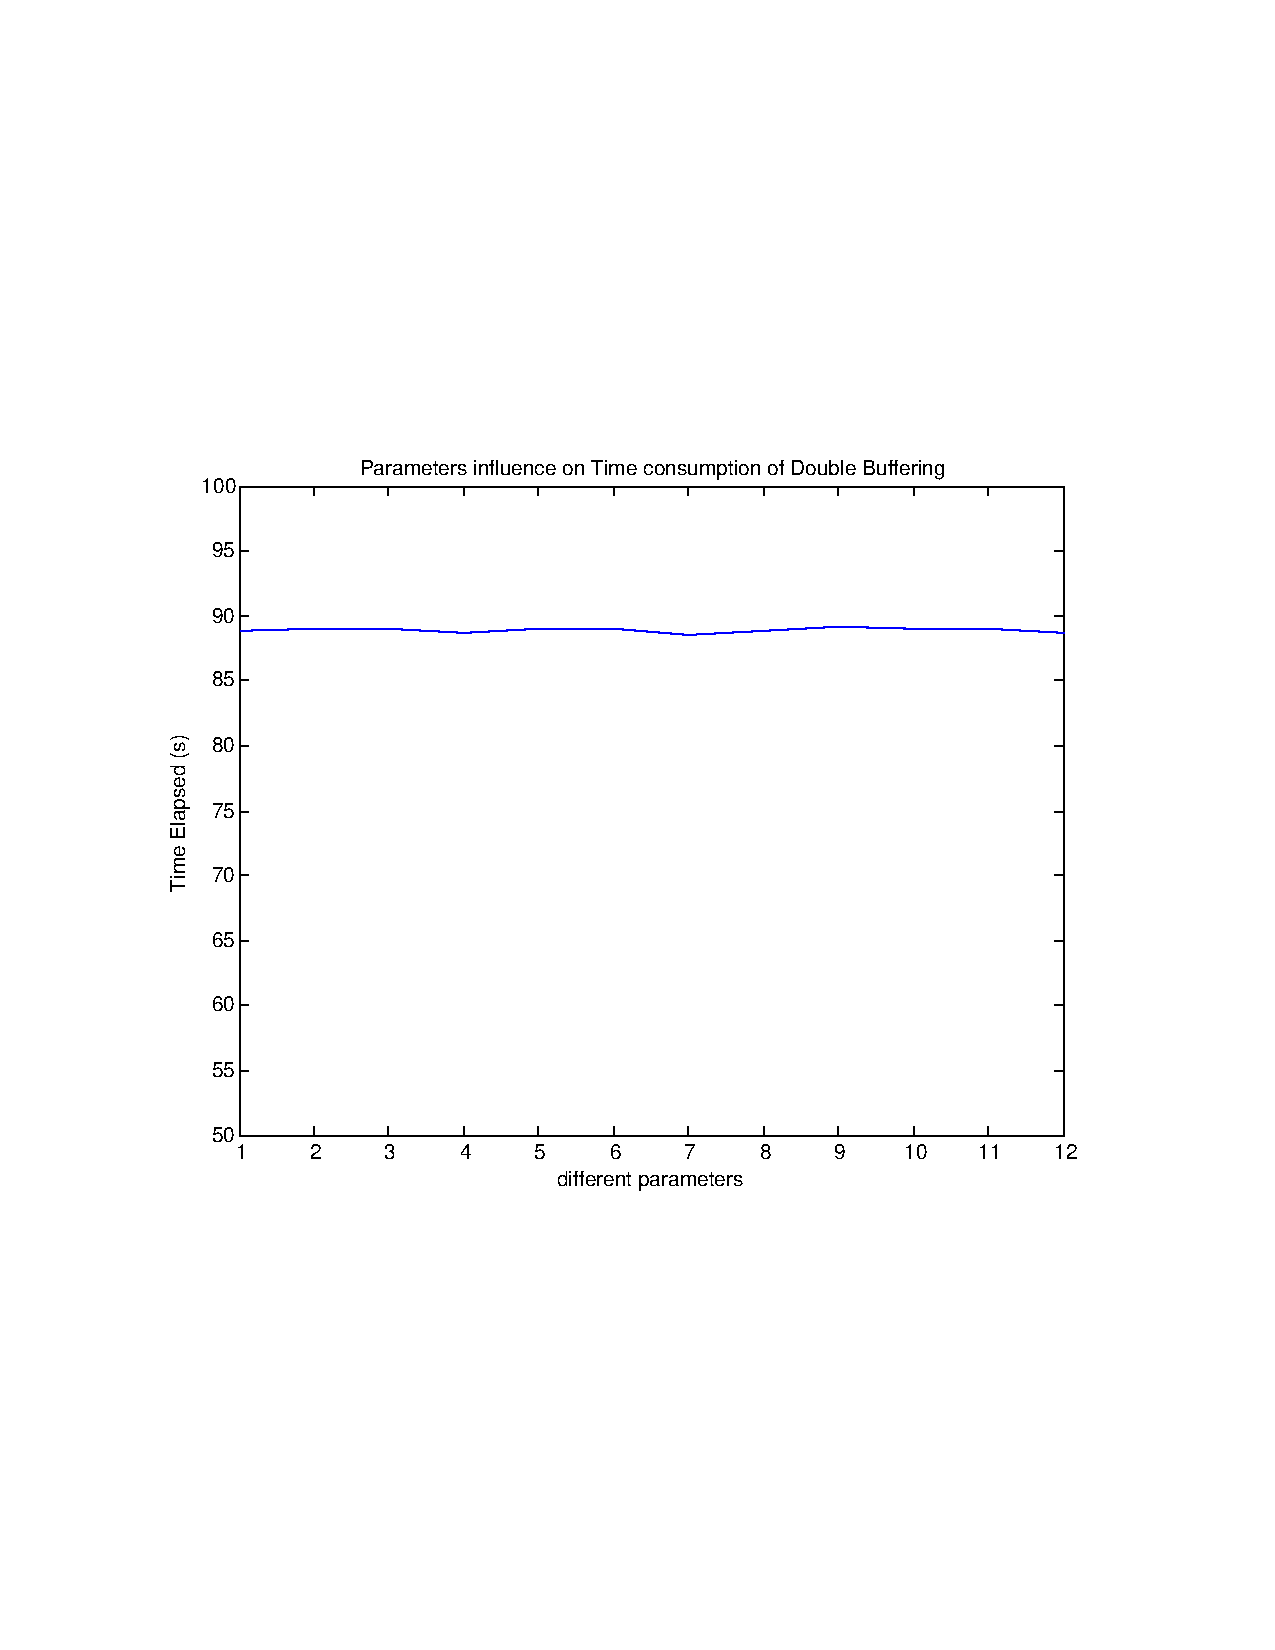
\includegraphics[width = \linewidth]{r_gpu42.pdf}
\caption{time consumption with the increase of matrix size}
\label{fig:rgpu41}
\end{figure}

\subsection{Result with the increase of matrix size}

In this part the time consumption is also determined by matrix size, tile\_width and task\_width. Tile\_width is chosen from $\{ 20, 30, 50, 100\}$ and task\_width is chosen from $\{2, 5, 10\}$. Figure 17 shows the fastest among these experiments, where $tile\_width = 30$ and $task\_width = 10$. Here the maximum matrix size is $30000 \times 30000$. However, the difference between time consumption of taking different parameters doesn't vary too much. For example, when the matrix size is $5000 \times 5000$ the time consumptions of taking different parameters are shown in Figure 18.  

\begin{figure}[hbp!]
\centering
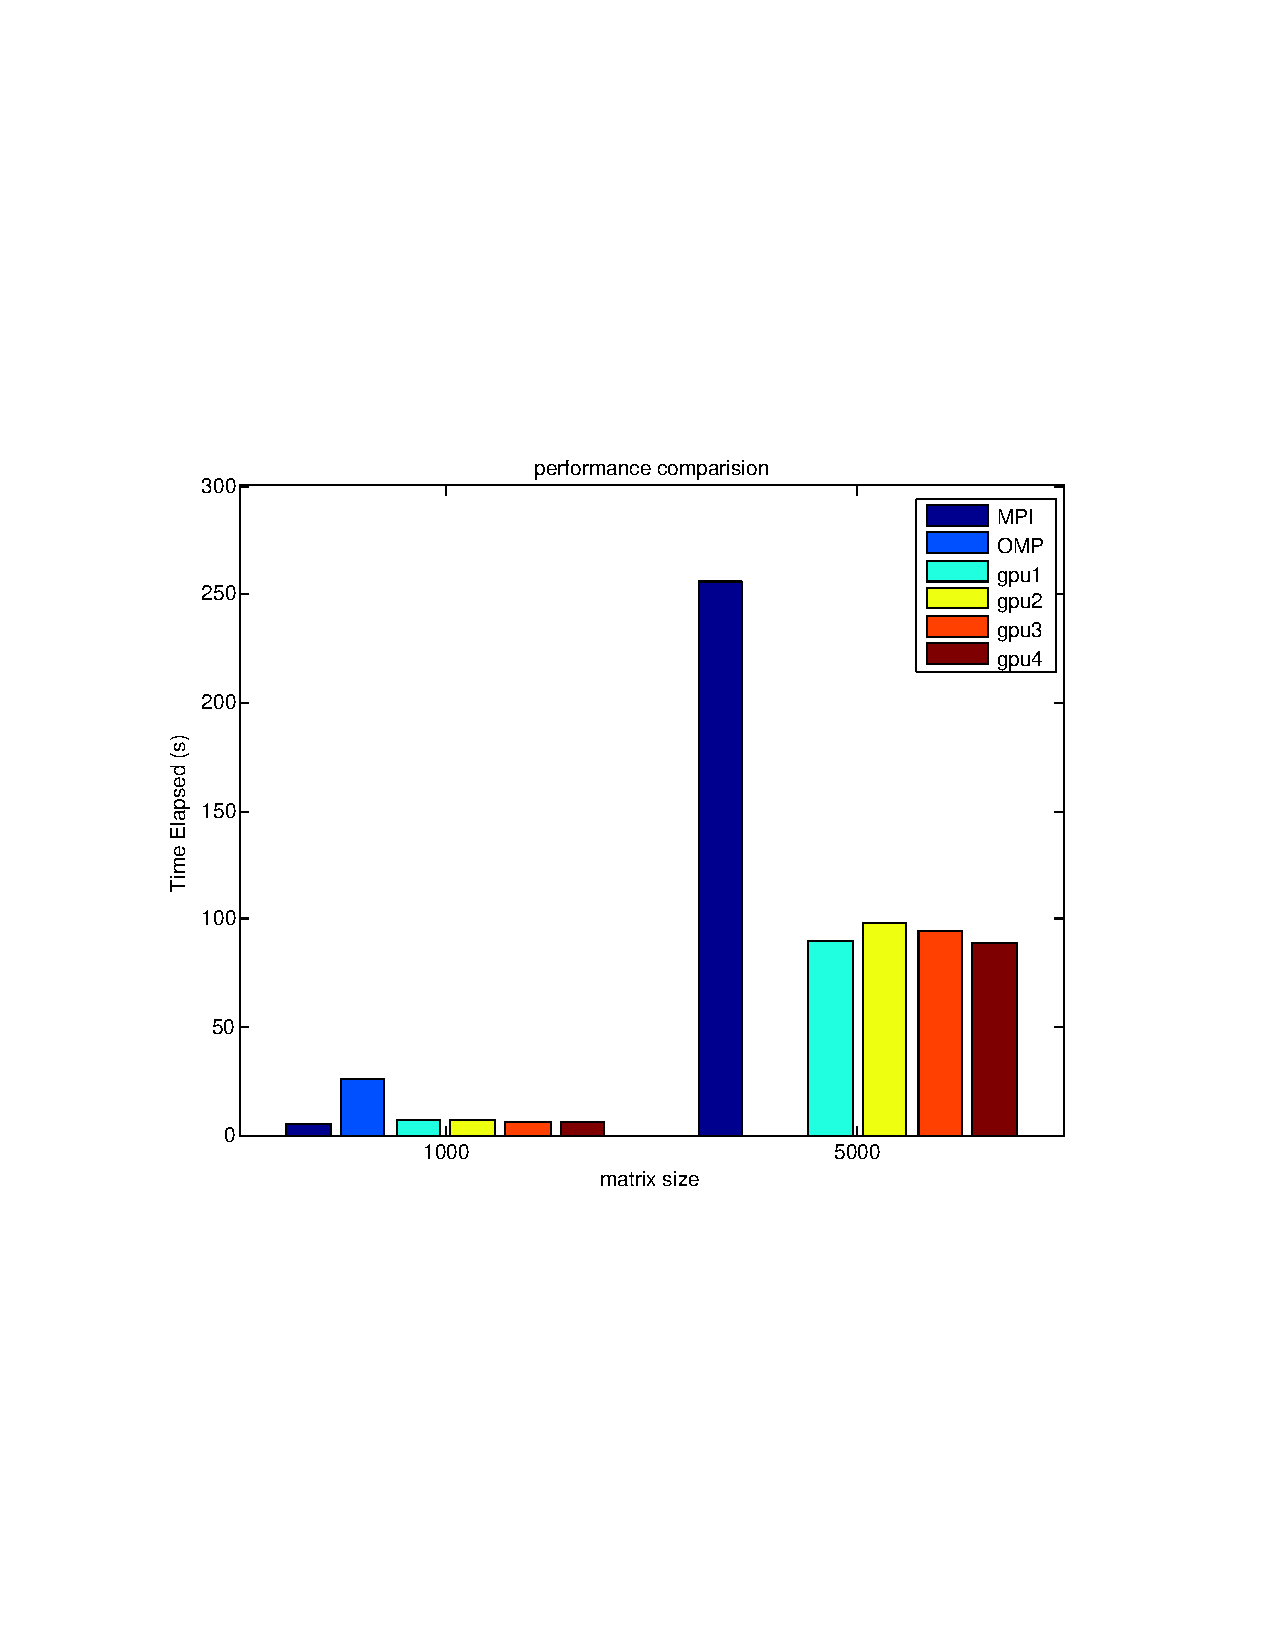
\includegraphics[width = \linewidth]{comp.pdf}
\caption{comparison with MPI, OpenMP and all the above methods.}
\label{fig:comp}
\end{figure}

\section{Comparison with MPI and OpenMP and all the above GPU paradigms}
Figure 19 shows the performance comparison with OpenMP and MPI when computing matrix size of $1000 \times 1000$ and $5000 \times 5000$. (Since the computational time of OpenMP for $5000 \times 5000$ matrix is too large to observe, the second group of bars misses one bar.) Here the MPI performance was observed when using 20 processors, OpenMP performance was observed using 20 processors, the $gpu1$ bar indicates the "One block with one thread per element" method, $gpu2$ indicates the "Multiple block with one thread per element" method, $gpu3$ indicates the "Multiple block with one thread multiple element" method and $gpu4$ indicates the "double buffering" method. The performance is chosen when each method performs the best in experiment. For GPU methods, the computational time of their maximum matrix size, which is $30000\times 30000$, are nearly equal with each other. 

\end {document}
